\documentclass[final,hyperref={pdfpagelabels=false}]{beamer}
\usepackage{grffile}
\usepackage{ragged2e}
\mode<presentation>
  {
  %  \usetheme{Berlin}
  \usetheme{I6pd2}
  }
  \usepackage{times}
  \usepackage{amsmath,amsthm, amssymb, latexsym}
  \boldmath
  \usepackage[english]{babel}
  \usepackage[latin1]{inputenc}
  \usepackage[orientation=portrait,size=custom,width=80,height=120,scale=1.4]{beamerposter}  
  
  % my packages 
  \usepackage{multirow} 

  %%%%%%%%%%%%%%%%%%%%%%%%%%%%%%%%%%%%%%%%%%%%%%%%%%%%%%%%%%%%%%%%%%%%%%%%%%%%%%%%%5
  \graphicspath{{figures/}}
  \title[Fancy Posters]{Verification of Translation Model Transformations\\\vspace{.5cm}Validity and Completeness Results}

  \author[Dreuw \& Deselaers]{Levi L\'ucio$^{\dagger}$, Bentley James Oakes$^{\dagger}$, and Hans Vangheluwe$^{\ddagger\dagger}$}
    
    \institute[McGill University]{$^{\dagger}$McGill University, Montreal,
    Canada\qquad $^{\ddagger}$University of Antwerp, Belgium}
  
  \date[June 14th, 2011]{\today}
  
  %%%%%%%%%%%%%%%%%%%%%%%%%%%%%
  \begin{document}
  \begin{frame}{} 
     \vspace{-1.5cm}
      \begin{columns}[t]
        \begin{column}{.993\linewidth}
        \begin{block}{\large Problem Statement}\vspace{.5cm}
 Our transformation verification approach employs a technique inspired from
 symbolic execution in order to automatically build a set of path
 conditions for a DSLTrans transformation~\cite{MODELS2010,SLE2010}. Each path condition abstractly represents a number of concrete
 transformation executions. Based on this formally defined abstraction relation, we show that \textbf{our path condition
 generation algorithm is both \emph{valid} and \emph{complete}}.
   		
 Using \textbf{path conditions}, we are then able to prove model syntax relation properties over all transformation
 executions in a model-independent way.
 This is done by examining if the properties hold on the set of path conditions.
 Through the \textbf{abstraction relation}, if the property does not hold on a path
 condition, the property will not hold on the transformation executions
 abstracted by the path condition. We show \textbf{this property proving step is
 both \emph{valid} and \emph{complete}}.\vspace{1cm}
        \end{block}
        \end{column}
      \end{columns}         
 
	
	 \begin{columns}[t]
	   \begin{column}{.71\linewidth}
        \begin{block}{Main Artifacts in Model Transformation Verification}
        \begin{columns}[c]
       \begin{column}{.50\linewidth}
       \begin{center}
         \textbf{DSLTrans Transformation:}\vspace{2cm}
         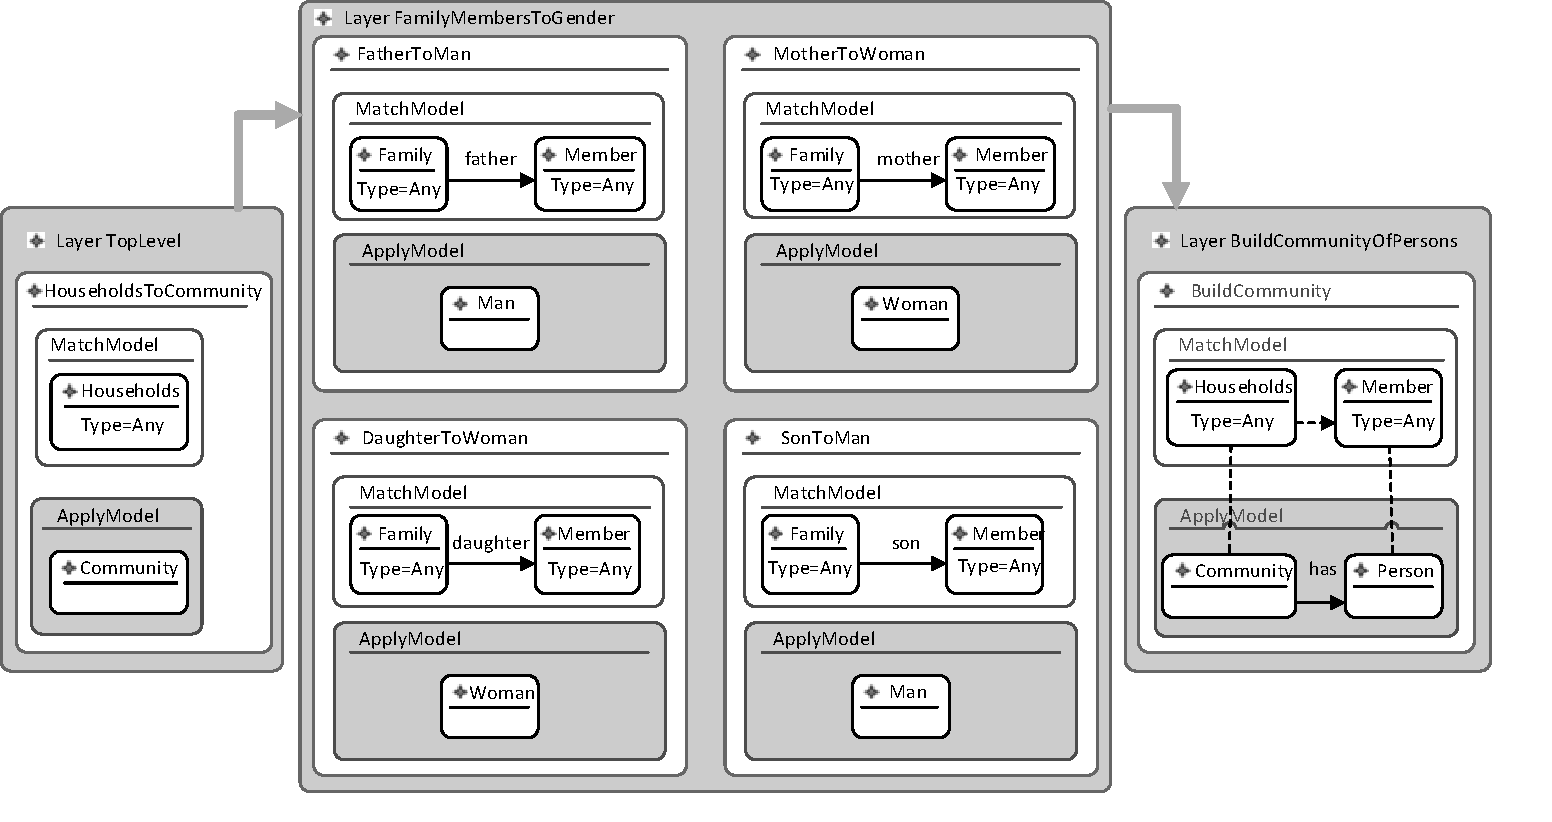
\includegraphics[width=.9\textwidth]{../figures/presentation/artifacts/transformation}\\
         \vspace{.7cm}\footnotesize{
         Six rules arranged in three layers that execute sequentially.  
         Each rule is composed of a Match Model and an Apply Model, analogous to the LHS and RHS in other transformation formalisms.\vspace{1cm}}
         \end{center}
         \end{column}
         \vrule{}
               \begin{column}{.24\linewidth}
               \begin{center}
          \vspace{-1cm}\textbf{Property:}\vspace{1cm}
            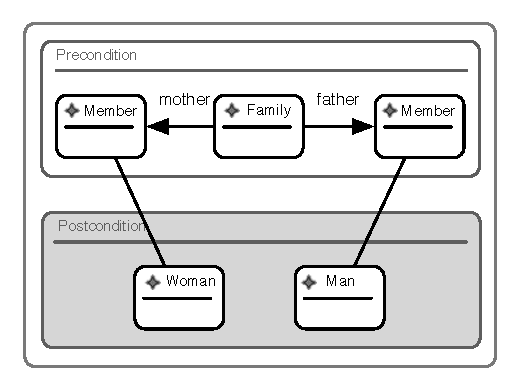
\includegraphics[width=\textwidth]{../figures/presentation/artifacts/property}\\
            %\vspace{.5cm}
            \small{Model Syntax Relation\\ \emph{AtomicContract} with\\pre- and post- conditions} \\\vspace{1cm}\footnotesize{``the mother and father in a family will always be transformed into a woman
            and a man''} 
            \end{center}
            \end{column} 
            \vrule{} 
        \begin{column}{.24\linewidth}
        \begin{center} 
          \vspace{-1.5cm}\textbf{Transformation\\ Execution:}\vspace{0.5cm}
          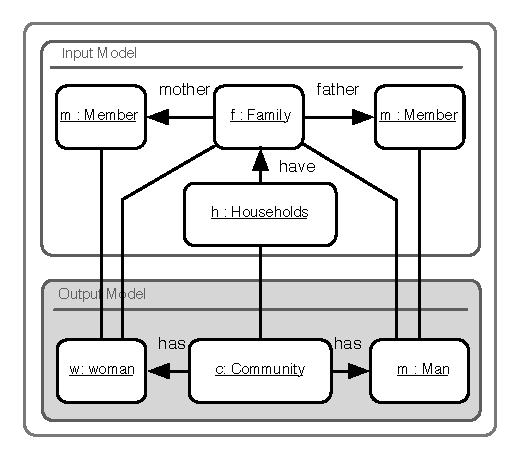
\includegraphics[width=.99\textwidth]{../figures/presentation/artifacts/trans_ex}\\
          \vspace{0.5cm}\small{Input and resulting Output}\\\vspace{1.2cm}\footnotesize{\textit{Traceability links} record which output elements were created from which input elements}
          \end{center} 
          \end{column} 
              \end{columns} 
        \end{block}
        \end{column}

        \begin{column}{.26\linewidth}

         \begin{block}{Proving Properties}
         \vspace{1.5cm}
        \small{
        The aim of our procedure is to prove \emph{model syntax relation}
        properties on all transformation executions. However, as there are
        \textbf{infinitely many transformation executions}, the proof requires
        an \textbf{abstraction}.\\~\\
		\vspace{.5cm}
        \textbf{Path conditions} abstract transformation executions. A path condition represents a combination of rules of the transformation that can execute. In a path condition each rule is represented only once, granting the required abstraction and ensuring the generation of a finite number of path conditions.} 
        \vspace{1.55cm}
%         Through the abstraction relation shown below \textbf{the set of path conditions generated for a DSLTrans transformation represents all possible executions of that transformation given an arbitrary input model}.
        \end{block}
        \end{column}
       \end{columns}
      
      

      \begin{columns}[t]
        \begin{column}{.993\linewidth}      
			\begin{block}{Abstraction Relation}
                \begin{columns}[t]
                \begin{column}{.24\linewidth}
                \begin{center}
              
                
                \textbf{Example Path Condition:}\\
              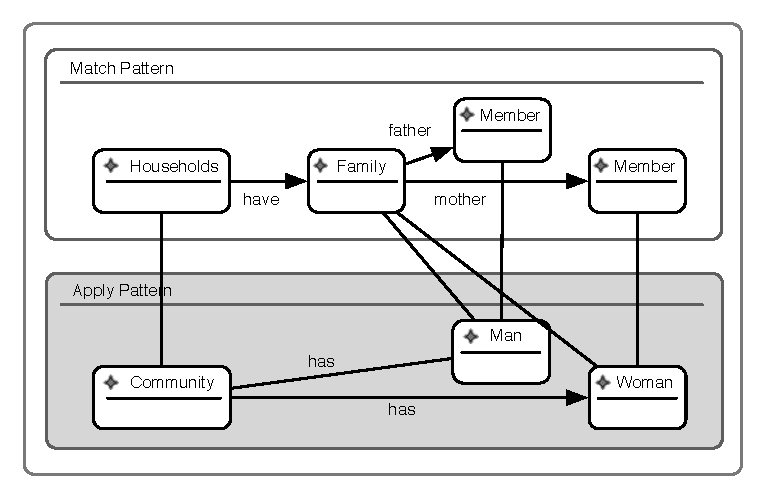
\includegraphics[width=0.8\textwidth]{../figures/presentation/artifacts/path_condition}\\
            
             \footnotesize{Path conditions are created by combining transformation rules~\cite{LuVa2013a}}\vspace{1cm}
                                  
%              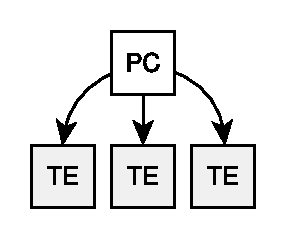
\includegraphics[width=0.7\textwidth]{../figures/presentation/abstraction_relation}\\
%              One path condition can abstract many transformation executions
             
              \end{center}            
              \small{
              A \textbf{Path Condition} \emph{abstracts} a transformation execution when:}
              \vspace{.2cm}
              \begin{itemize}
                \item \small{An \textbf{\emph{Injective Typed Graph Homomorphism}} exists between the match part of each rule (component) in the path condition and the input of the transformation execution, \textbf{and}}\vspace{.5cm}
                \item \small{A \textbf{\emph{Surjective Typed Graph Homomorphism}} exists between the output of the transformation execution (including traceability links) and the apply graph of the path condition.}
              \end{itemize}
                           
              \end{column}
              \vrule{}
              \begin{column}{.65\linewidth}
%               \large
%               \begin{center}
%              \textbf{\normalsize{Abstraction Holds}}\\
%               \end{center}
%              
%              \normalsize
%               
%               \begin{column}{.5\linewidth} 
%                \begin{center}
%                     \textbf{Empty Path Condition:}\\
%                  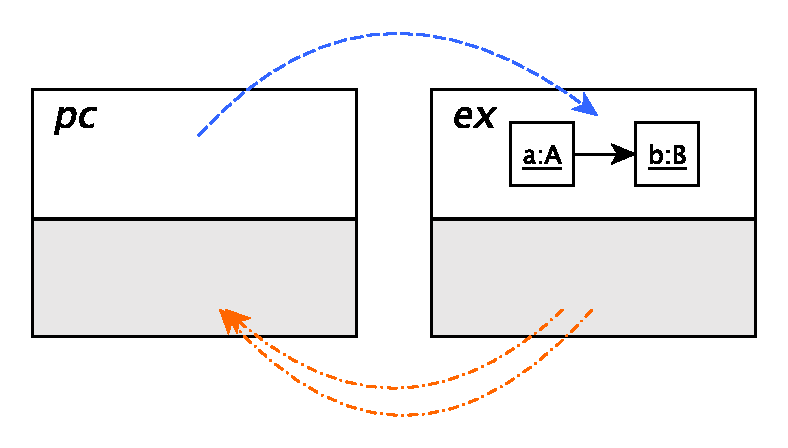
\includegraphics[width=\textwidth]{../figures/presentation/abstraction_relation/empty_pc}
%                 
%                                  
%                      \textbf{Non-Overlapping Rules:}\\
%                   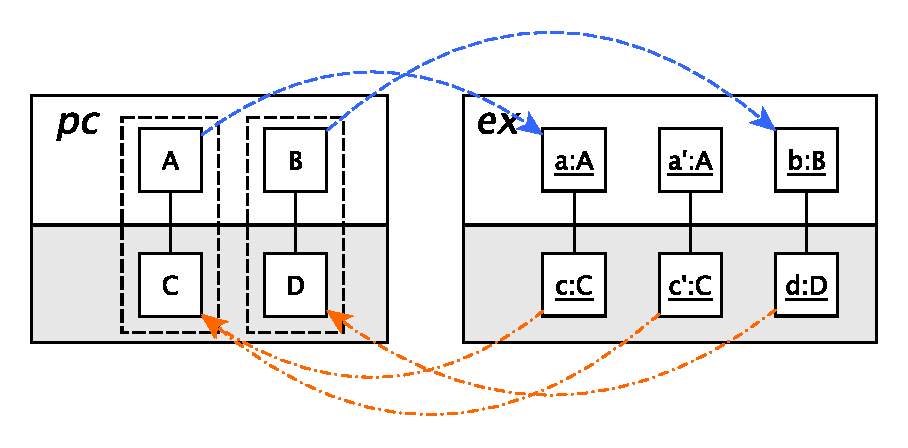
\includegraphics[width=\textwidth]{../figures/presentation/abstraction_relation/non_overlapping2}
%                   
%                    \end{center} 
%                  \end{column}
%                  \begin{column}{.5\linewidth}
%                   \begin{center}
%                    \textbf{Non-Overlapping Rules:}\\
%                                      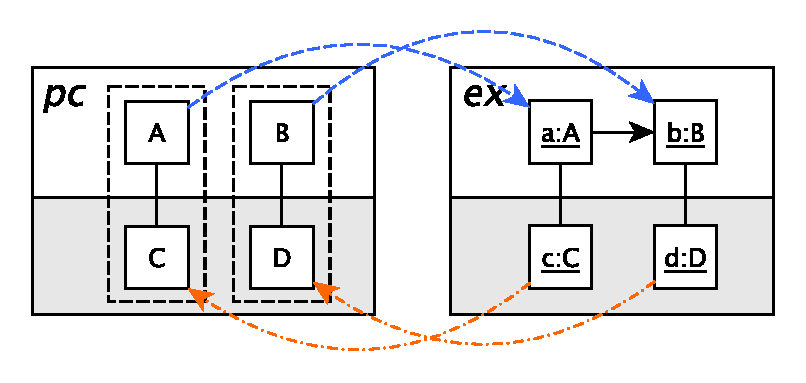
\includegraphics[width=\textwidth]{../figures/presentation/abstraction_relation/non_overlapping}
%                    
%                  
%                   \textbf{Overlapping Rules:}\\
%  	            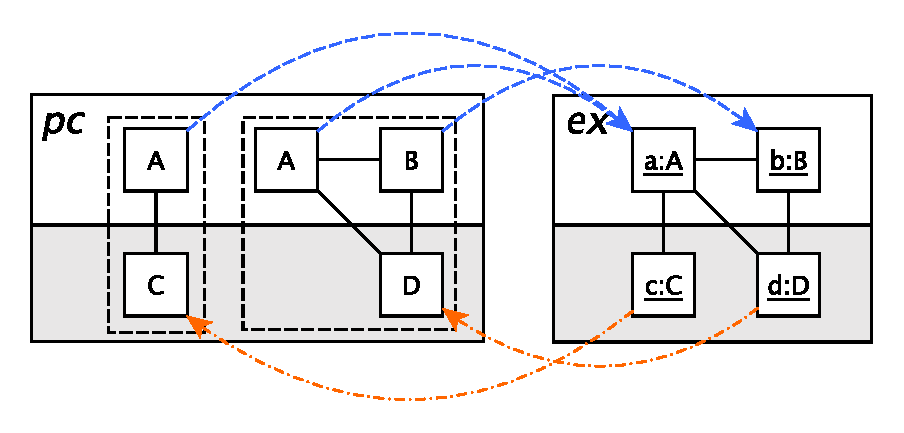
\includegraphics[width=\textwidth]{../figures/presentation/abstraction_relation/overlapping}
%  	            
%  	            \end{center} 
%                 \end{column}
%                 
%                    \begin{center}
% %                   \textbf{Given this abstraction relation, properties that are proven on a path condition will hold on all transformation executions which the path condition abstracts over}
%                		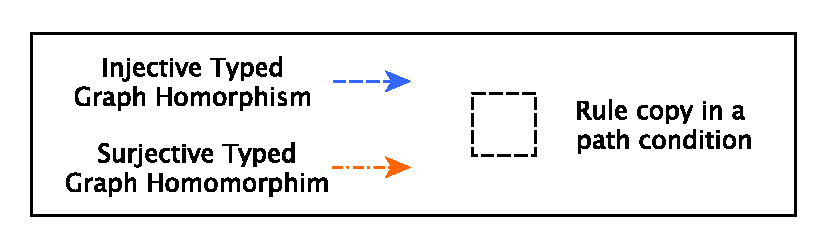
\includegraphics[width=0.3\textwidth]{../figures/abstraction_relation/legend}                   
%                    \end{center}
%                  
%                    \end{column}
%                   \vrule{}
%                   \begin{column}{.24\linewidth}
%                    \begin{center}
%                    
%                    \large
%                    \textbf{\normalsize{Abstraction Does Not Hold}}
%                    \normalsize
%                    
%                   \textbf{Empty Path Condition:}\\
%                   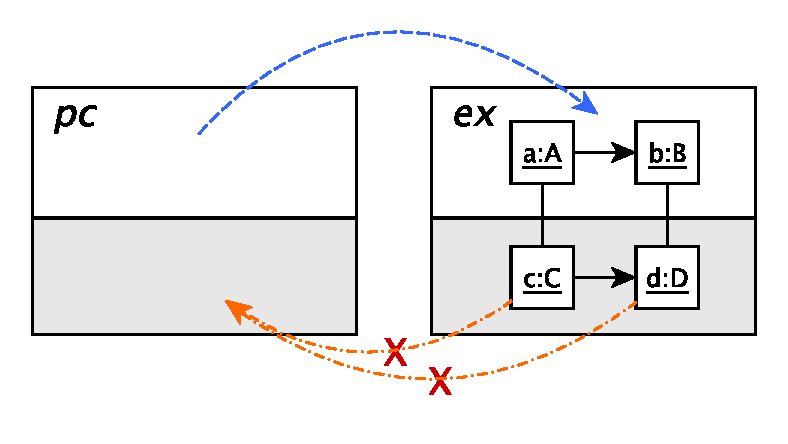
\includegraphics[width=\textwidth]{../figures/presentation/abstraction_relation/empty_pc2}
%                   
%                   Surjective typed graph homomorphism does not hold
%                                          
%                     
%                         \textbf{Overlapping Rules:}\\
%         	            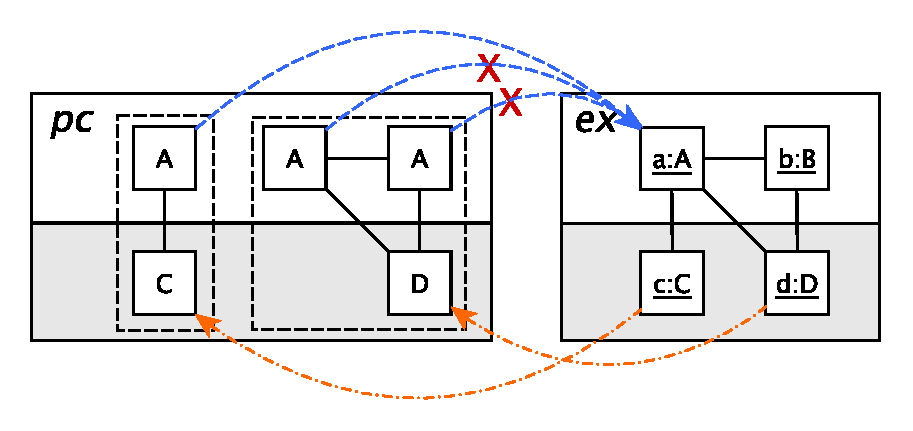
\includegraphics[width=\textwidth]{../figures/presentation/abstraction_relation/overlapping2}
%         	            
%         	            Injective typed graph homomorphism does not hold
%                         \end{center} 

              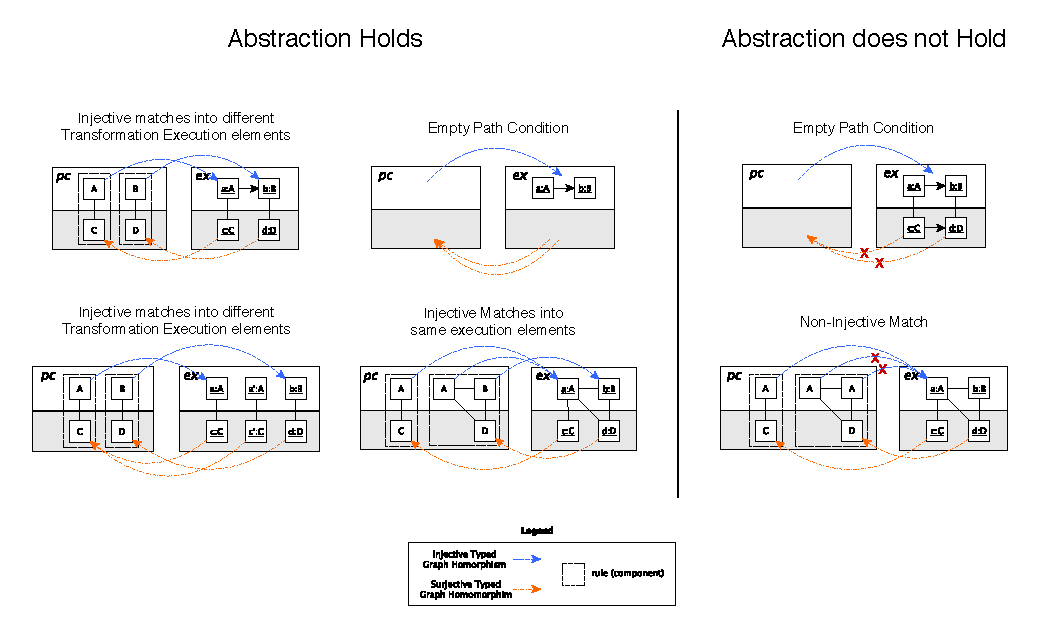
\includegraphics[width=1\textwidth]{../figures/presentation/abstraction_relation/abstraction}\\

                    \end{column}
                 \end{columns}
%                 \vspace{1cm}
                \end{block}
      		\end{column}
        \end{columns}  
                
%   \vspace{-1.5cm}
   \begin{columns}[t]
                   \begin{column}{.485\linewidth}
                   
			\begin{block}{Path Condition Generation Validity/Completeness Theorems~\cite{LuVa2013a}}
                \begin{columns}[t]
                \begin{column}{.4\linewidth}
              \textbf{Validity:}
              \small{Every path condition abstracts at least one transformation execution.}
              
              \end{column}
              \hspace{-2cm}
			  \vrule{} 
              \hspace{1cm}
                            
              \begin{column}{.485\linewidth}
                  \textbf{Completeness:}
                    \small{Every transformation execution is abstracted by one
                    path condition.}
                 \end{column}                            
                 \end{columns} 
                 \vspace{0.5cm} 
%			  	 \hrule{}  
                 \vspace{0.5cm} 
                 \small{\textbf{Uniqueness:}}
                 \footnotesize{Every transformation execution is abstracted by \textbf{\textit{exactly}} one
                 path condition.}              
                 
                \end{block}   
                
                \end{column} 
                \begin{column}{.485\linewidth}
       \begin{block}{Property Proving Validity/Completeness Theorems~\cite{LuVa2013a}}
                       \begin{columns}[t]
                       \begin{column}{.485\linewidth}
                     \textbf{Validity:}
                     \small{Checking a property on a path condition and on a transformation execution that path condition abstracts produces the same result.}
                     \end{column}
              		 \hspace{-2cm}                     
                     \vrule{}
               		 \hspace{.3cm}
                     \begin{column}{.485\linewidth}
                          \textbf{Completeness:}
                        \small{A property can be proved to hold or not hold on all transformation executions.}
      					\vspace{1.93cm} 
                        \end{column}
                       \end{columns}
                       \end{block}                    
      \end{column}
      \end{columns}
   
  
   \begin{columns}[t] 
    \begin{column}{.485\linewidth}
    	\begin{block}{Future Work}
   	   \begin{itemize}
   	   \item Integrate in the theory the treatment of rules whose match graphs are subgraphs of other rules (already in the tool).
   	   \item Integrate contract negation in the theory (already in the tool).
   	   \item Integrate negative application conditions (NACs) into our symbolic verification approach.
   	   \item Expand expressiveness of the property language by allowing properties that involve multiple applications of the same rule.
   	   \end{itemize}
        \end{block}
        
    \end{column}
    \begin{column}{.485\linewidth}
    	\begin{block}{Bibliography}
    	   \footnotesize
    	   \begin{thebibliography}{10}   
    	   \bibitem{MODELS2010} Levi L\'ucio, Bruno Barroca, Vasco Amaral, {\em A
    	   Technique for Automatic Validation of Model Transformations},
    	   Proceedings of the MoDELS 2010 Conference, Springer, pp. 136-150.
    	   \bibitem{SLE2010} Bruno Barroca, Levi L\'ucio, Vasco Amaral, Roberto
    	   F{\'e}lix and Vasco Sousa, {\em DSLTrans: A Turing Incomplete
    	   Transformation Language}, Proceedings of the SLE 2010 conference,
    	   Springer 2010, pp. 296-305.
 		   \bibitem{LuVa2013a} Levi L\'ucio, Bentley Oakes and Hans Vangheluwe, {\em A Technique for Symbolically Verifying Properties of Graph-Based Model Transformations},  Technical Report SOCS-TR-2014.1, McGill University, 2013.
		\vspace{1.65cm}
		\end{thebibliography}	   
    	\end{block}        
    \end{column}    
   \end{columns}

  \end{frame}
\end{document}